\documentclass[border=10pt]{standalone}
\usepackage{tikz}
\usepackage{amsmath} % For \hat and \boldsymbol
\usetikzlibrary{shapes.geometric, arrows.meta, positioning, calc}

\begin{document}
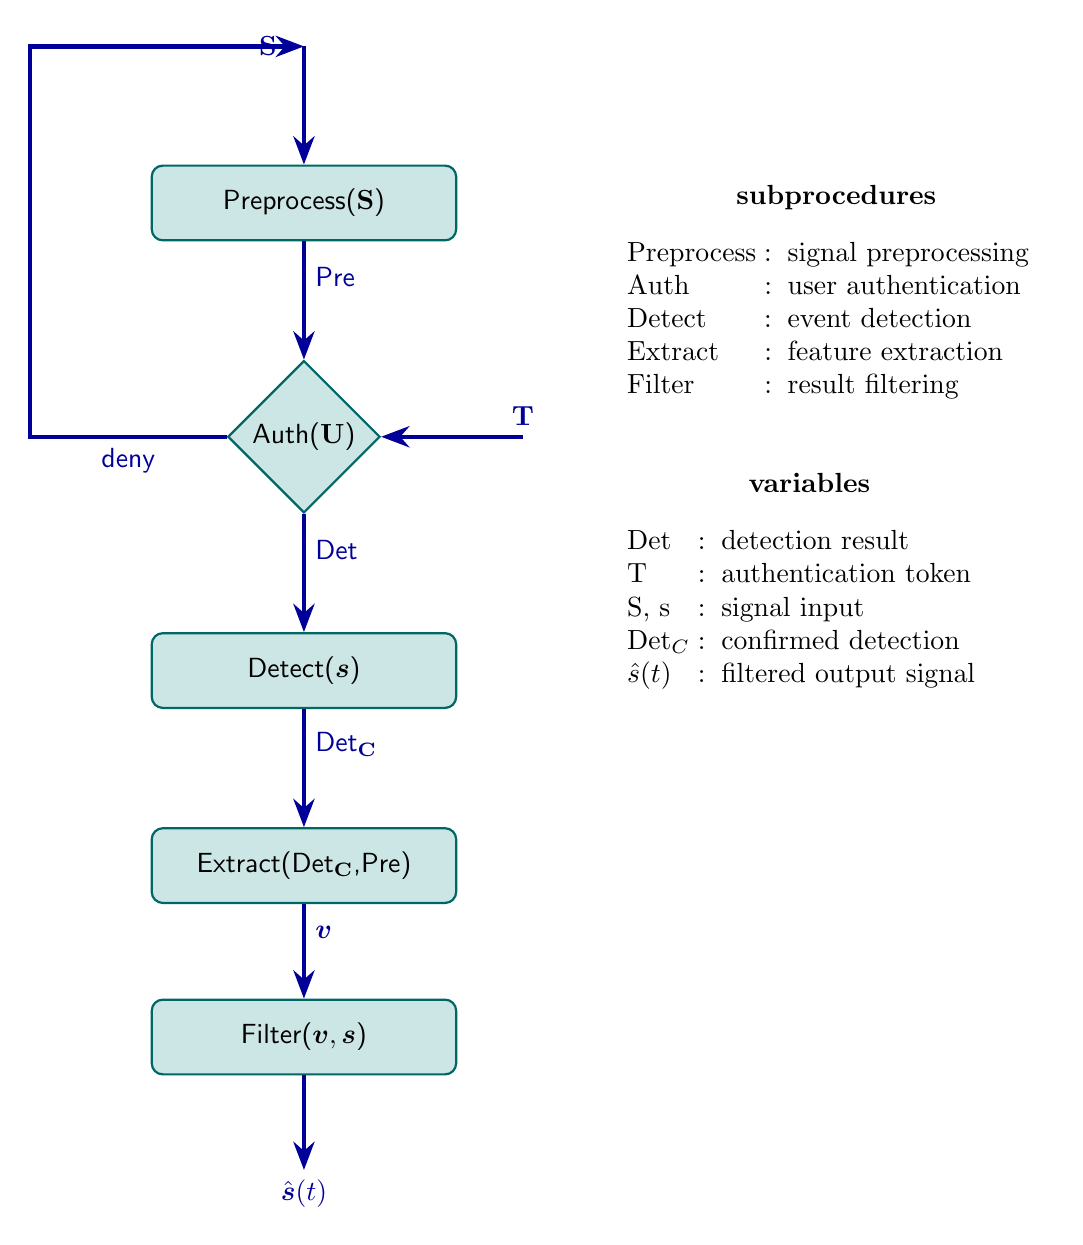
\begin{tikzpicture}[
    % Define colors
    myblue/.style={color=blue!60!black},
    mycyanfill/.style={fill=teal!20},
    mycyanborder/.style={draw=teal!80!black},
    % Define node styles
    process/.style={
        rectangle,
        rounded corners,
        mycyanborder,
        mycyanfill,
        thick,
        minimum height=2.7em,
        minimum width=11em,
        text centered,
        font=\sffamily
    },
    decision/.style={
        diamond,
        mycyanborder,
        mycyanfill,
        thick,
        minimum size=5.5em,
        aspect=1.5,
        text centered,
        inner sep=0pt,
        font=\sffamily
    },
    % Define arrow style
    arrow/.style={
        ->,
        ultra thick,
        myblue,
        >=Stealth
    },
    % Style for labels on arrows
    label/.style={
        myblue,
        font=\sffamily
    }
]

% --- Flowchart Nodes ---
% Using 'node distance' for consistent spacing
\node[process] (preprocess) {Preprocess($\mathbf{S}$)};
\node[decision] (auth) [below=1.5cm of preprocess] {Auth($\mathbf{U}$)};
\node[process] (detect) [below=1.5cm of auth] {Detect($\boldsymbol{s}$)};
\node[process] (extract) [below=1.5cm of detect] {Extract(Det$_{\mathbf{C}}$,Pre)};
\node[process] (filter) [below=1.2cm of extract] {Filter($\boldsymbol{v},\boldsymbol{s}$)};
\node (s_hat) [below=1.2cm of filter, label] {$\hat{\boldsymbol{s}}(t)$};

% --- Input/Output points and arrows ---
\coordinate (S_target) at ($(preprocess.north)+(0,1.5cm)$);
\draw[arrow] (S_target) node[label, left=2mm] {$\mathbf{S}$} -- (preprocess);
\draw[arrow] (preprocess) -- (auth) node[pos=0.3, right, label] {Pre};
\draw[arrow] ($(auth.east)+(1.8cm,0)$) node[label, above] {$\mathbf{T}$} -- (auth);
\draw[arrow] (auth) -- (detect) node[pos=0.3, right, label] {Det};
\draw[arrow] (detect) -- (extract) node[pos=0.3, right, label] {Det$_{\mathbf{C}}$};
\draw[arrow] (extract) -- (filter) node[pos=0.3, right, label] {$\boldsymbol{v}$};
\draw[arrow] (filter) -- (s_hat);

% --- Feedback Loop ---
\draw[arrow] (auth.west) -- ++(-2.5,0) node[midway, below, label] {deny} |- (S_target);

% --- Text Blocks on the right ---
\node (text_block) [right=3cm of auth, align=left, anchor=west] {
    \begin{tabular}{@{}l @{\hspace{1mm}:\hspace{2mm}} l}
    \multicolumn{2}{c}{\bfseries subprocedures} \\[3mm]
    Preprocess & signal preprocessing \\
    Auth & user authentication \\
    Detect & event detection \\
    Extract & feature extraction \\
    Filter & result filtering \\
    \end{tabular}
    \\[8mm]
    \begin{tabular}{@{}l @{\hspace{1mm}:\hspace{2mm}} l}
    \multicolumn{2}{c}{\bfseries variables} \\[3mm]
    Det & detection result \\
    T & authentication token \\
    S, s & signal input \\
    Det$_C$ & confirmed detection \\
    $\hat{s}(t)$ & filtered output signal \\
    \end{tabular}
};

\end{tikzpicture}
\end{document}
